\documentclass{standalone}
\usepackage{tikz}
\usetikzlibrary{patterns, positioning}

\begin{document}
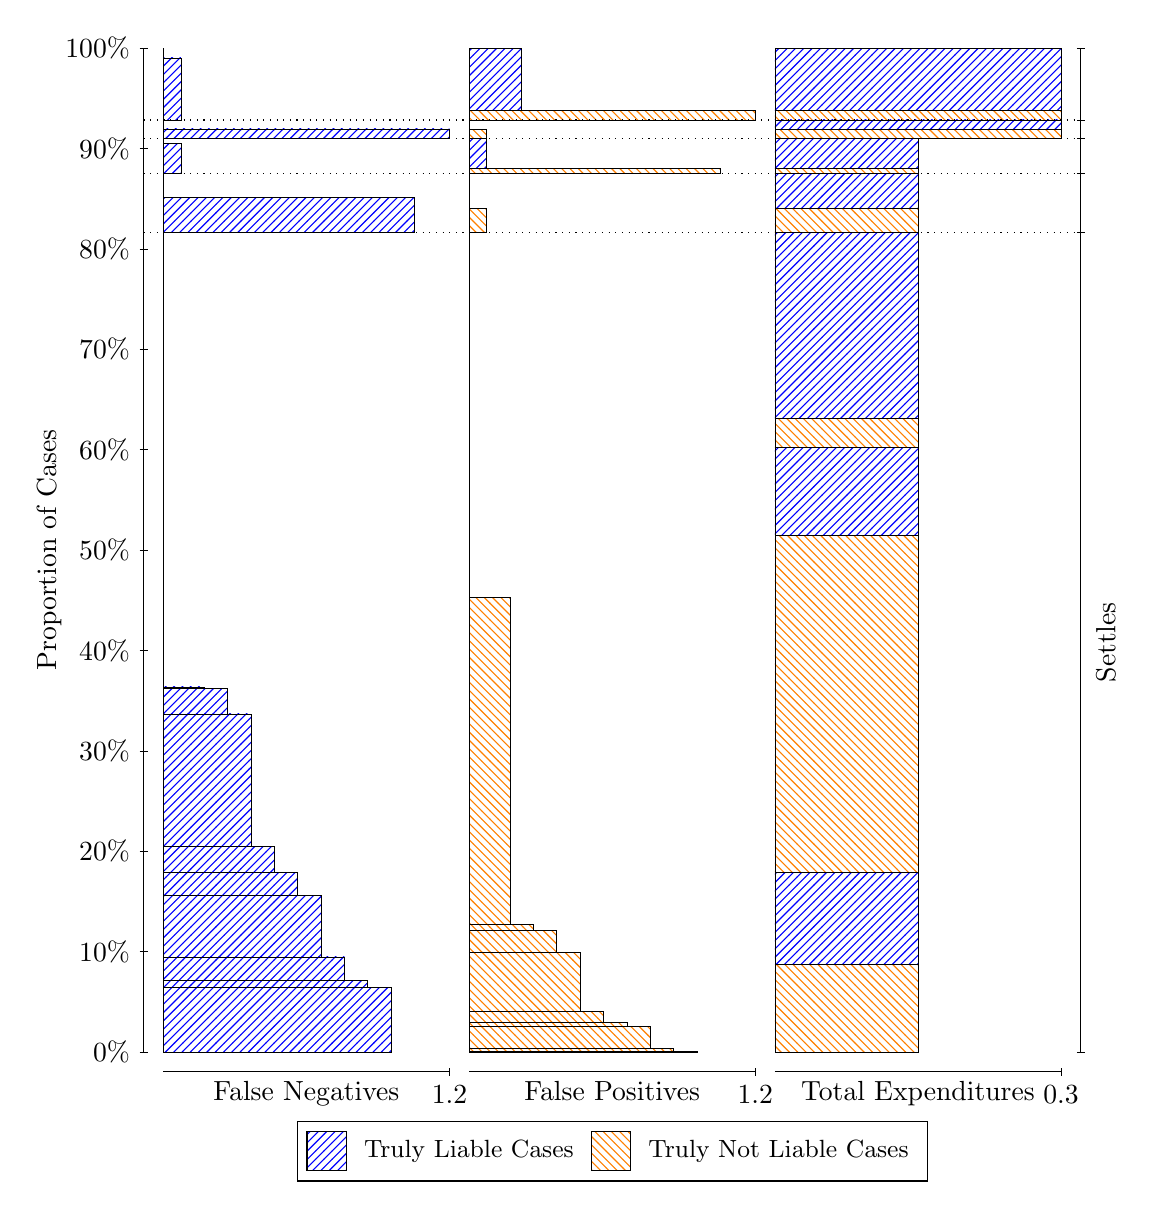
\begin{tikzpicture}
\draw[black, very thin] (1.5,1.75) -- (1.5,14.5);
\node[rotate=90, anchor=center] at (0.3, 8.125) {Proportion of Cases};
\draw[black, very thin] (1.45,1.75) -- (1.55,1.75);
\node[anchor=east] at (1.45, 1.75) {0\%};
\draw[black, very thin] (1.45,3.025) -- (1.55,3.025);
\node[anchor=east] at (1.45, 3.025) {10\%};
\draw[black, very thin] (1.45,4.3) -- (1.55,4.3);
\node[anchor=east] at (1.45, 4.3) {20\%};
\draw[black, very thin] (1.45,5.575) -- (1.55,5.575);
\node[anchor=east] at (1.45, 5.575) {30\%};
\draw[black, very thin] (1.45,6.85) -- (1.55,6.85);
\node[anchor=east] at (1.45, 6.85) {40\%};
\draw[black, very thin] (1.45,8.125) -- (1.55,8.125);
\node[anchor=east] at (1.45, 8.125) {50\%};
\draw[black, very thin] (1.45,9.4) -- (1.55,9.4);
\node[anchor=east] at (1.45, 9.4) {60\%};
\draw[black, very thin] (1.45,10.675) -- (1.55,10.675);
\node[anchor=east] at (1.45, 10.675) {70\%};
\draw[black, very thin] (1.45,11.95) -- (1.55,11.95);
\node[anchor=east] at (1.45, 11.95) {80\%};
\draw[black, very thin] (1.45,13.225) -- (1.55,13.225);
\node[anchor=east] at (1.45, 13.225) {90\%};
\draw[black, very thin] (1.45,14.5) -- (1.55,14.5);
\node[anchor=east] at (1.45, 14.5) {100\%};

\draw[black, very thin] (13.4,1.75) -- (13.4,14.5);
\draw[black, very thin] (13.35,1.75) -- (13.45,1.75);
\node[anchor=west] at (13.35, 1.75) {};
\draw[black, very thin] (13.35,12.157) -- (13.45,12.157);
\node[anchor=west] at (13.35, 12.157) {};
\draw[black, very thin] (13.35,12.906) -- (13.45,12.906);
\node[anchor=west] at (13.35, 12.906) {};
\draw[black, very thin] (13.35,13.351) -- (13.45,13.351);
\node[anchor=west] at (13.35, 13.351) {};
\draw[black, very thin] (13.35,13.586) -- (13.45,13.586);
\node[anchor=west] at (13.35, 13.586) {};
\draw[black, very thin] (13.35,14.5) -- (13.45,14.5);
\node[anchor=west] at (13.35, 14.5) {};

\draw[black, very thin, pattern color=blue, pattern=north east lines] (1.75,1.75) rectangle (4.6418,2.5663);
\draw[black, very thin, pattern color=blue, pattern=north east lines] (1.75,2.5663) rectangle (4.3452,2.6612);
\draw[black, very thin, pattern color=blue, pattern=north east lines] (1.75,2.6612) rectangle (4.0486,2.9576);
\draw[black, very thin, pattern color=blue, pattern=north east lines] (1.75,2.9576) rectangle (3.752,3.7357);
\draw[black, very thin, pattern color=blue, pattern=north east lines] (1.75,3.7357) rectangle (3.4554,4.0296);
\draw[black, very thin, pattern color=blue, pattern=north east lines] (1.75,4.0296) rectangle (3.1588,4.3614);
\draw[black, very thin, pattern color=blue, pattern=north east lines] (1.75,4.3614) rectangle (2.8622,6.0438);
\draw[black, very thin, pattern color=blue, pattern=north east lines] (1.75,6.0438) rectangle (2.5656,6.3627);
\draw[black, very thin, pattern color=blue, pattern=north east lines] (1.75,6.3627) rectangle (2.269,6.3856);
\draw[black, very thin, pattern color=orange, pattern=north west lines] (1.75,6.3856) rectangle (1.75,12.157);
\draw[black, very thin, pattern color=blue, pattern=north east lines] (1.75,12.157) rectangle (4.9384,12.604);
\draw[black, very thin, pattern color=orange, pattern=north west lines] (1.75,12.604) rectangle (1.75,12.906);
\draw[black, very thin, pattern color=blue, pattern=north east lines] (1.75,12.906) rectangle (1.9724,13.288);
\draw[black, very thin, pattern color=orange, pattern=north west lines] (1.75,13.288) rectangle (1.75,13.351);
\draw[black, very thin, pattern color=blue, pattern=north east lines] (1.75,13.351) rectangle (5.3833,13.474);
\draw[black, very thin, pattern color=orange, pattern=north west lines] (1.75,13.474) rectangle (1.75,13.586);
\draw[black, very thin, pattern color=blue, pattern=north east lines] (1.75,13.586) rectangle (1.9724,14.374);
\draw[black, very thin, pattern color=orange, pattern=north west lines] (1.75,14.374) rectangle (1.75,14.5);
\draw[black, very thin, pattern color=orange, pattern=north west lines] (5.6333,1.75) rectangle (8.5252,1.754);
\draw[black, very thin, pattern color=orange, pattern=north west lines] (5.6333,1.754) rectangle (8.2286,1.7994);
\draw[black, very thin, pattern color=orange, pattern=north west lines] (5.6333,1.7994) rectangle (7.932,2.0709);
\draw[black, very thin, pattern color=orange, pattern=north west lines] (5.6333,2.0709) rectangle (7.6354,2.1265);
\draw[black, very thin, pattern color=orange, pattern=north west lines] (5.6333,2.1265) rectangle (7.3388,2.2641);
\draw[black, very thin, pattern color=orange, pattern=north west lines] (5.6333,2.2641) rectangle (7.0422,2.2688);
\draw[black, very thin, pattern color=orange, pattern=north west lines] (5.6333,2.2688) rectangle (7.0422,3.013);
\draw[black, very thin, pattern color=orange, pattern=north west lines] (5.6333,3.013) rectangle (6.7456,3.2897);
\draw[black, very thin, pattern color=orange, pattern=north west lines] (5.6333,3.2897) rectangle (6.449,3.3726);
\draw[black, very thin, pattern color=orange, pattern=north west lines] (5.6333,3.3726) rectangle (6.1524,7.5214);
\draw[black, very thin, pattern color=blue, pattern=north east lines] (5.6333,7.5214) rectangle (5.6333,12.157);
\draw[black, very thin, pattern color=orange, pattern=north west lines] (5.6333,12.157) rectangle (5.8558,12.459);
\draw[black, very thin, pattern color=blue, pattern=north east lines] (5.6333,12.459) rectangle (5.6333,12.906);
\draw[black, very thin, pattern color=orange, pattern=north west lines] (5.6333,12.906) rectangle (8.8218,12.97);
\draw[black, very thin, pattern color=blue, pattern=north east lines] (5.6333,12.97) rectangle (5.8558,13.351);
\draw[black, very thin, pattern color=orange, pattern=north west lines] (5.6333,13.351) rectangle (5.8558,13.464);
\draw[black, very thin, pattern color=blue, pattern=north east lines] (5.6333,13.464) rectangle (5.6333,13.586);
\draw[black, very thin, pattern color=orange, pattern=north west lines] (5.6333,13.586) rectangle (9.2667,13.712);
\draw[black, very thin, pattern color=blue, pattern=north east lines] (5.6333,13.712) rectangle (6.3007,14.5);
\draw[black, very thin, pattern color=orange, pattern=north west lines] (9.5167,1.75) rectangle (11.333,2.8585);
\draw[black, very thin, pattern color=blue, pattern=north east lines] (9.5167,2.8585) rectangle (11.333,4.0279);
\draw[black, very thin, pattern color=orange, pattern=north west lines] (9.5167,4.0279) rectangle (11.333,8.3143);
\draw[black, very thin, pattern color=blue, pattern=north east lines] (9.5167,8.3143) rectangle (11.333,9.4244);
\draw[black, very thin, pattern color=orange, pattern=north west lines] (9.5167,9.4244) rectangle (11.333,9.8009);
\draw[black, very thin, pattern color=blue, pattern=north east lines] (9.5167,9.8009) rectangle (11.333,12.157);
\draw[black, very thin, pattern color=orange, pattern=north west lines] (9.5167,12.157) rectangle (11.333,12.459);
\draw[black, very thin, pattern color=blue, pattern=north east lines] (9.5167,12.459) rectangle (11.333,12.906);
\draw[black, very thin, pattern color=orange, pattern=north west lines] (9.5167,12.906) rectangle (11.333,12.97);
\draw[black, very thin, pattern color=blue, pattern=north east lines] (9.5167,12.97) rectangle (11.333,13.351);
\draw[black, very thin, pattern color=orange, pattern=north west lines] (9.5167,13.351) rectangle (13.15,13.464);
\draw[black, very thin, pattern color=blue, pattern=north east lines] (9.5167,13.464) rectangle (13.15,13.586);
\draw[black, very thin, pattern color=orange, pattern=north west lines] (9.5167,13.586) rectangle (13.15,13.712);
\draw[black, very thin, pattern color=blue, pattern=north east lines] (9.5167,13.712) rectangle (13.15,14.5);
\draw[black, dotted] (1.5,12.157) -- (13.4,12.157);
\draw[black, dotted] (1.5,12.906) -- (13.4,12.906);
\draw[black, dotted] (1.5,13.351) -- (13.4,13.351);
\draw[black, dotted] (1.5,13.586) -- (13.4,13.586);
\draw[black, very thin] (1.75,1.5) -- (5.3833,1.5);
\node[anchor=north] at (3.5667, 1.5) {False Negatives};
\draw[black, very thin] (5.3833,1.45) -- (5.3833,1.55);
\node[anchor=north] at (5.3833, 1.45) {1.2};

\draw[black, very thin] (5.6333,1.5) -- (9.2667,1.5);
\node[anchor=north] at (7.45, 1.5) {False Positives};
\draw[black, very thin] (9.2667,1.45) -- (9.2667,1.55);
\node[anchor=north] at (9.2667, 1.45) {1.2};

\draw[black, very thin] (9.5167,1.5) -- (13.15,1.5);
\node[anchor=north] at (11.333, 1.5) {Total Expenditures};
\draw[black, very thin] (13.15,1.45) -- (13.15,1.55);
\node[anchor=north] at (13.15, 1.45) {0.3};

\node[black, centered, rotate=90] at (13.72, 6.9535) {Settles};





\draw (7.449999999999999,1.5) node[draw=none] (baseCoordinate) {};
\begin{scope}[align=center]
        \matrix[scale=0.5, draw=black, below=0.5cm of baseCoordinate, nodes={draw}, column sep=0.1cm]{
            \node[rectangle, draw, minimum width=0.5cm, minimum height=0.5cm, pattern=north east lines, pattern color=blue] {}; &
            \node[draw=none, font=\small] (B) {Truly Liable Cases}; &
            \node[rectangle, draw, minimum width=0.5cm, minimum height=0.5cm, pattern=north west lines, pattern color=orange] {}; &
            \node[draw=none, font=\small] (B) {Truly Not Liable Cases}; \\
            };
\end{scope}

\end{tikzpicture}
\end{document}